\documentclass[11pt]{article}

\usepackage[margin=0.88in]{geometry}
\usepackage[T1]{fontenc}
\usepackage{lmodern}
\usepackage{microtype}
\usepackage{graphicx}
\usepackage{amsmath,amssymb}
\usepackage{booktabs}
\usepackage{array}
\usepackage{threeparttable}
\usepackage{enumitem}
\usepackage{float}
\usepackage{xcolor}
\usepackage{xurl}
\usepackage[hidelinks]{hyperref}
\usepackage[font=small,labelfont=bf]{caption}
\usepackage{authblk}
\usepackage{fancyhdr}
\usepackage{titlesec}
\usepackage{tikz}
\usepackage{pgfplots}
\usepgfplotslibrary{groupplots}
\usetikzlibrary{arrows.meta,positioning,shapes.geometric}
\pgfplotsset{compat=1.18}

\definecolor{navy}{HTML}{17324D}
\hypersetup{
  colorlinks=true,
  linkcolor=navy,
  citecolor=navy,
  urlcolor=navy,
  pdftitle={Extending BioNeuralNet with Leiden and Embedding-Refined Community Detection for Multi-Omics Feature Module Discovery},
  pdfauthor={Muhammad Babar, Md Abu Sufian, Nadeem Qazi, N. Berardinelli, Tasmia Umme Jannat},
  pdfkeywords={multi-omics, graph neural networks, Leiden, community detection, TCGA-BRCA, BioNeuralNet}
}
\setlist{nosep,leftmargin=1.4em}
\setlength{\parindent}{1.2em}
\setlength{\parskip}{0.15em}
\renewcommand{\arraystretch}{1.15}
\captionsetup{justification=justified,singlelinecheck=false}
\titleformat{\section}{\large\bfseries\color{navy}}{\thesection}{0.65em}{}
\titleformat{\subsection}{\normalsize\bfseries}{\thesubsection}{0.65em}{}
\titlespacing*{\section}{0pt}{1.5ex plus .4ex}{0.7ex}
\titlespacing*{\subsection}{0pt}{1.1ex plus .3ex}{0.45ex}
\pagestyle{fancy}
\fancyhf{}
\fancyhead[L]{\footnotesize BioNeuralNet Leiden extension}
\fancyhead[R]{\footnotesize Babar et al.}
\fancyfoot[C]{\thepage}
\setlength{\headheight}{14pt}

\title{\textbf{Extending BioNeuralNet with Leiden and Embedding-Refined Community Detection for Multi-Omics Feature Module Discovery}}
\author[1]{Muhammad Babar}
\author[2]{Md Abu Sufian\thanks{Corresponding author: Md Abu Sufian; \href{mailto:m.sufian@uel.ac.uk}{m.sufian@uel.ac.uk}.}}
\author[3]{Nadeem Qazi}
\author[4]{N. Berardinelli}
\author[5]{Tasmia Umme Jannat}
\affil[1]{Department of Computer Science, University of Colorado Denver, Denver, CO, USA; \href{mailto:muhammad.babar@ucdenver.edu}{muhammad.babar@ucdenver.edu}}
\affil[2]{Department of Computer Science, University of East London, London E16 2RD, UK; \href{mailto:m.sufian@uel.ac.uk}{m.sufian@uel.ac.uk}}
\affil[3]{Department of Engineering and Computing, School of Architecture, Computing and Engineering, University of East London, London E16 2RD, UK; \href{mailto:N.Qazi@uel.ac.uk}{N.Qazi@uel.ac.uk}}
\affil[4]{Department of Computer Science and Digital Technologies, School of Architecture, Computing and Engineering, University of East London, London E16 2RD, UK; \href{mailto:N.Berardinelli@uel.ac.uk}{N.Berardinelli@uel.ac.uk}}
\affil[5]{Barts Cancer Institute, Queen Mary University of London, London EC1M 6AU, UK; \href{mailto:t.jannat@qmul.ac.uk}{t.jannat@qmul.ac.uk}}
\renewcommand{\Authfont}{\normalsize\bfseries}
\renewcommand{\Affilfont}{\small\itshape}
\setlength{\affilsep}{0.45em}
\date{}

\begin{document}
\maketitle

\begin{abstract}
Network-based multi-omics workflows require clustering methods that can preserve molecular graph topology while remaining flexible enough to resolve structure in learned embeddings. BioNeuralNet provides graph construction and graph neural network (GNN) representation learning, but its clustering interface has lacked a direct implementation of Leiden community detection with optional embedding-level refinement. This study adds a weighted Leiden component and a hybrid strategy that applies local K-means within sufficiently large Leiden communities. The implementation preserves node order during NetworkX-to-igraph conversion, supports weighted Reichardt--Bornholdt partitions, validates embedding dimensions, and exposes deterministic random-state control.

The extension was evaluated on 769 TCGA breast invasive carcinoma cases with 1,000 high-variance RNA features, 1,000 high-variance DNA-methylation features, and 503 miRNA features. A cosine 25-nearest-neighbour feature graph contained 2,503 nodes and 35,495 edges. A four-layer graph attention network generated 64-dimensional, PAM50-guided feature embeddings. At resolution 0.25, Leiden produced 12 modules; local K-means refinement produced 22. Refinement improved embedding-space dispersion (Davies--Bouldin index, 35.19 to 25.94) and slightly improved the silhouette coefficient (-0.085 to -0.061), but reduced weighted graph modularity (0.699 to 0.290) and raw-expression silhouette (0.025 to -0.123). In a secondary patient-clustering stress test, five-cluster K-means on 16-dimensional principal components achieved adjusted Rand index/normalized mutual information of 0.363/0.492, whereas default Leiden and hybrid settings over-partitioned the sparse patient graph and performed worse.

These results do not support universal superiority of the hybrid method. Instead, they establish a reproducible BioNeuralNet extension and identify an explicit resolution--fidelity trade-off: Leiden is preferable when graph coherence is primary, while local refinement is useful when finer embedding-space partitions are required and independently validated.
\end{abstract}

\noindent\textbf{Keywords:} multi-omics; feature networks; graph neural networks; graph attention networks; Leiden algorithm; community detection; TCGA-BRCA; BioNeuralNet

\medskip
\noindent\textbf{Article focus:} Software and methods development for graph-based multi-omics feature-module discovery.

\section{Introduction}

Breast cancer is molecularly heterogeneous, and clinically similar tumours may differ substantially in transcriptional, epigenetic, and post-transcriptional regulation. The PAM50 classifier captures major intrinsic expression subtypes, including luminal A, luminal B, HER2-enriched, basal-like, and normal-like disease \cite{parker2009,tcga2012}. These classes are useful reference labels, but they do not exhaust the continuous and multi-layered structure present in tumour profiles. Integrative analysis is therefore commonly used to identify molecular modules, patient groups, and cross-omic associations that are not evident from a single data layer.

Graphs provide a natural representation for this task. Nodes may represent molecular features or patients, and weighted edges can encode similarity, co-expression, or prior biological relationships. Similarity Network Fusion demonstrated that patient networks from distinct omics layers can support cancer stratification \cite{wang2014snf}; more recent GNN approaches learn nonlinear representations from such networks for classification and biomarker analysis \cite{wang2021mogonet,schultesasse2021}. BioNeuralNet consolidates these operations in a modular Python framework that supports network construction, GNN embeddings, subgraph detection, and downstream prediction \cite{ramos2026}. Its design makes it a suitable platform for testing clustering algorithms without rebuilding the surrounding multi-omics workflow.

Clustering a graph-derived representation is nevertheless an objective-dependent problem. K-means favours approximately convex groups in Euclidean space. Spectral methods use a graph Laplacian but still require a predefined number of clusters. Density-based methods are sensitive to heterogeneous density. Community-detection algorithms instead optimize a network quality function. Leiden is particularly attractive because it improves the local-moving and refinement stages of Louvain and guarantees connected communities under its stated conditions \cite{traag2019}. Yet a topological partition may be too coarse for a downstream task that emphasizes continuous GNN embeddings. Conversely, splitting a graph community using embedding geometry may improve local compactness while breaking graph coherence.

This work addresses that tension by extending BioNeuralNet with two related modes: weighted Leiden community detection and optional local K-means refinement inside Leiden communities. The contribution is methodological and software-oriented rather than a claim of a new breast cancer taxonomy. Specifically, the study:
\begin{enumerate}
    \item implements deterministic, weighted Leiden clustering with validated alignment between graph nodes and embedding rows;
    \item introduces a bounded local-refinement rule that preserves small communities and subdivides only large communities in embedding space; and
    \item evaluates the resulting trade-off using graph modularity, embedding and expression geometry, module--phenotype association, and a separate patient-clustering stress test.
\end{enumerate}

The analysis corrects an important conceptual ambiguity: the primary experiment clusters \emph{multi-omics features}, not patients. Patient clustering is reported separately and shows that parameters appropriate for a feature graph do not automatically transfer to patient stratification.

\section{Related Work}

Multi-omics integration methods broadly use latent-factor models, similarity networks, or deep representations. Similarity Network Fusion constructs one patient network per modality and iteratively combines them \cite{wang2014snf}. MOGONET uses modality-specific GCNs and cross-omic discovery for supervised classification and biomarker identification \cite{wang2021mogonet}. Other GNN methods integrate biological networks and molecular measurements to prioritize cancer-associated genes \cite{schultesasse2021}. These approaches motivate the use of graph structure, but their downstream partitions remain sensitive to graph construction and clustering objectives.

BioNeuralNet provides a general framework rather than a single disease model. Its molecular nodes may carry subject-level observations, engineered statistics, centrality features, phenotype associations, and learned embeddings \cite{ramos2026}. The framework already includes correlated and Louvain-related subgraph utilities. The present extension adds Leiden as a first-class option and permits a second-stage embedding refinement without changing BioNeuralNet's data-loading or representation-learning interfaces.

Leiden optimizes modularity-like objectives through local movement, partition refinement, and graph aggregation \cite{traag2019}. This study uses the Reichardt--Bornholdt configuration-model objective \cite{reichardt2006},
\begin{equation}
Q_{\gamma}(\mathcal{C}) = \sum_{c\in\mathcal{C}}
\left(e_c - \gamma\frac{K_c^2}{2m}\right),
\label{eq:rb}
\end{equation}
where $e_c$ is the total within-community edge weight, $K_c$ is the weighted degree sum in community $c$, $m$ is total edge weight, and $\gamma$ controls resolution. The proposed hybrid does not redefine this objective. It treats the Leiden partition as a topology-preserving first level and then applies K-means to embedding vectors within selected communities. Consequently, its final partition is not expected to maximize Eq.~\ref{eq:rb}; the empirical comparison explicitly measures the resulting loss of graph coherence.

\section{Materials and Methods}

\subsection{Study design and reproducibility}

The complete workflow is shown in Figure~\ref{fig:workflow}. The primary analysis uses molecular features as graph nodes and patients as observations. A secondary analysis transposes this orientation and uses patients as nodes. All reported values were regenerated from BioNeuralNet version 1.2.1 source at commit \texttt{3c1915dc62851875672636e91f04f1eb9f1faf81}. NumPy, PyTorch, GNN initialization, Leiden, K-means, PCA, and UMAP were assigned random state 42 where supported. The GNN was trained on CPU for 100 epochs. Results represent one deterministic run and are not presented as estimates over repeated resampling.

\begin{figure}[t]
    \centering
    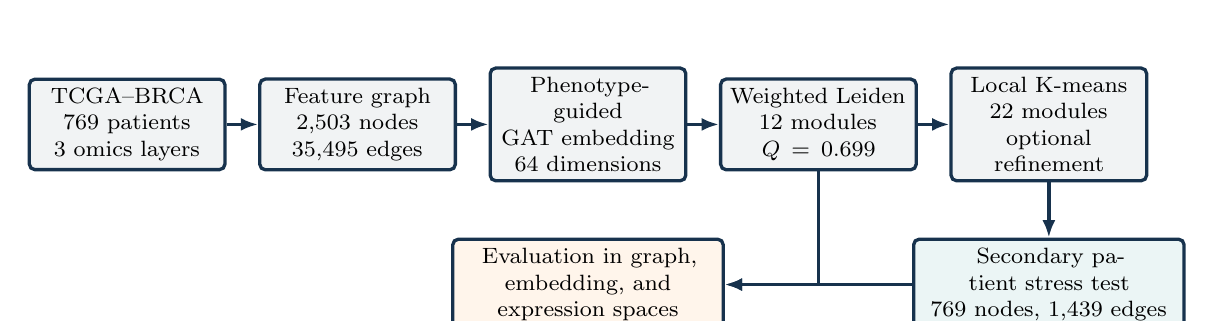
\begin{tikzpicture}[
      font=\footnotesize,
      box/.style={draw=navy,very thick,rounded corners=2pt,align=center,
        minimum height=1.05cm,text width=2.25cm,fill=navy!6},
      arrow/.style={-{Latex[length=2.2mm]},very thick,draw=navy}
    ]
      \node[box] (data) {TCGA--BRCA\\769 patients\\3 omics layers};
      \node[box,right=4mm of data] (graph) {Feature graph\\2,503 nodes\\35,495 edges};
      \node[box,right=4mm of graph] (gat) {Phenotype-guided\\GAT embedding\\64 dimensions};
      \node[box,right=4mm of gat] (lei) {Weighted Leiden\\12 modules\\$Q=0.699$};
      \node[box,right=4mm of lei] (hyb) {Local K-means\\22 modules\\optional refinement};
      \draw[arrow] (data)--(graph);
      \draw[arrow] (graph)--(gat);
      \draw[arrow] (gat)--(lei);
      \draw[arrow] (lei)--(hyb);
      \node[box,below=7mm of gat,text width=3.2cm,fill=orange!8] (eval)
        {Evaluation in graph, embedding, and expression spaces};
      \node[box,below=7mm of hyb,text width=3.2cm,fill=teal!8] (stress)
        {Secondary patient stress test\\769 nodes, 1,439 edges};
      \draw[arrow] (lei.south) |- (eval.east);
      \draw[arrow] (hyb.south) -- (stress.north);
      \draw[arrow] (stress.west) -- (eval.east);
    \end{tikzpicture}
    \caption{Evaluation workflow. The primary task clusters molecular features from three omics layers. Leiden supplies a weighted topological partition; optional local K-means subdivides eligible communities in the GAT embedding space.}
    \label{fig:workflow}
\end{figure}

\subsection{TCGA-BRCA cohort}

The processed TCGA-BRCA cohort distributed with BioNeuralNet contains 769 patients shared across RNA expression, DNA methylation, miRNA expression, clinical annotations, and PAM50 labels. Molecular data originate from TCGA/Firehose processing and PAM50 annotations from TCGAbiolinks-compatible subtype data. The five-class distribution is imbalanced, with luminal A accounting for 419 of 769 cases (Table~\ref{tab:data}). This imbalance is relevant to external clustering metrics and to any phenotype-guided representation.

\begin{table}[t]
\centering
\caption{Data used in the reproducible analysis.}
\label{tab:data}
\begin{threeparttable}
\small
\begin{tabular}{p{0.21\textwidth}p{0.22\textwidth}p{0.45\textwidth}}
\toprule
Component & Available dimensions & Used in analysis \\
\midrule
RNA expression & $769\times2{,}500$ & 1,000 highest-variance features \\
DNA methylation & $769\times2{,}203$ & 1,000 highest-variance features \\
miRNA expression & $769\times503$ & all 503 features \\
PAM50 label & $769\times1$ & LumA 419; Her2 46; LumB 140; Basal 130; Normal 34 \\
Clinical annotations & $769\times103$ & not used in the reported model \\
\bottomrule
\end{tabular}
\begin{tablenotes}[flushleft]\footnotesize
\item Rows are aligned patients. The numerical PAM50 mapping in the distributed data is LumA=0, Her2=1, LumB=2, Basal=3, and Normal=4.
\end{tablenotes}
\end{threeparttable}
\end{table}

BioNeuralNet's variance-selection utility replaces non-finite values, applies median imputation where required, removes zero-variance columns, and ranks numeric features by population variance. The selected RNA, methylation, and miRNA tables were concatenated column-wise to form a $769\times2{,}503$ matrix $X$. No additional modality weighting was used in the primary notebook design.

\subsection{Feature-similarity graph}

Each molecular feature was represented by its measurements across 769 patients. For feature vectors $x_i$ and $x_j$, cosine similarity was
\begin{equation}
s_{ij}=\frac{x_i^{\mathsf T}x_j}{\lVert x_i\rVert_2\lVert x_j\rVert_2}.
\end{equation}
The top $k=25$ neighbours of every feature were retained without requiring mutual neighbourhood membership. Self-loops were excluded, and outgoing similarities were row-normalized by the BioNeuralNet graph utility. The adjacency matrix was converted to an undirected NetworkX graph by preserving the upper-triangular positive edges and their weights. The resulting graph contained 2,503 nodes and 35,495 edges. A preliminary notebook sweep considered $k\in\{15,20,25\}$, mutual and non-mutual variants, and Leiden resolutions $\{0.10,0.25,0.50,1.00\}$. The reported $k=25$, non-mutual, $\gamma=0.25$ setting was selected exploratorily to avoid the extreme fragmentation observed in mutual graphs; it was not selected in a nested validation procedure.

\subsection{Phenotype-guided GAT feature embeddings}

BioNeuralNet's \texttt{GNNEmbedding} class produced a six-dimensional input vector for every molecular node: standardized mean, signed log-skewness, median absolute deviation, PageRank, eigenvector centrality, and Katz centrality. A four-layer graph attention network (GAT) \cite{velickovic2018} with hidden dimension 64, ReLU activation, dropout 0.5, and a scalar regression head was trained with Adam (learning rate $10^{-3}$; weight decay $10^{-4}$). Mean-squared error was minimized for 100 epochs, with early-stopping patience 50; the final training loss was 0.1909. The 64-dimensional penultimate-layer activations were used as node embeddings.

The regression target for each feature was BioNeuralNet's standardized Fisher transformation of the Pearson correlation between that feature and the numerically encoded PAM50 label. Thus, the primary embeddings are \emph{phenotype guided}, not unsupervised. Because PAM50 is nominal and its integer mapping imposes an arbitrary ordering, this target is a pragmatic software test rather than an ideal categorical association statistic. Module--PAM50 tests below are therefore descriptive checks of retained signal, not independent validation.

\subsection{Leiden and hybrid clustering extension}

The new \texttt{Leiden} class converts a NetworkX graph to igraph while retaining a fixed node order. It validates that an optional embedding matrix has one row per node, checks finite edge weights, and calls \texttt{leidenalg.find\_partition} with the weighted \texttt{RBConfigurationVertexPartition}. Leiden used edge weights, resolution 0.25, and seed 42.

The hybrid procedure starts from the Leiden labels. A community with at most 30 nodes is retained unchanged. For a larger community $c$ of size $n_c$, local K-means uses
\begin{equation}
k_c=\min\left(3,\max\left(1,\left\lfloor n_c/10\right\rfloor\right)\right).
\end{equation}
Eligible communities in the reported analysis therefore receive at most three embedding-derived submodules. K-means used 10 initializations and random state 42. New labels were assigned sequentially, with a final check that every graph node received exactly one label.

\subsection{Software interface and verification}

The extension is implemented as a reusable \texttt{Leiden} class rather than notebook-only code. Its constructor accepts a NetworkX graph, an optional node-embedding matrix, a switch for edge-weight use, a resolution parameter, and a random state. Instantiation creates the igraph representation and the base Leiden partition; \texttt{run(refine\_with\_kmeans=False)} returns an independent copy of the Leiden labels, whereas refinement requires an embedding matrix aligned to the stored node order. This interface separates the topology-first partition from the optional embedding-space operation and makes the selected mode explicit at the call site.

The accompanying test module exercises seven behaviours: NetworkX-to-igraph conversion with default weights, label-copy semantics without refinement, graphs with no edges, rejection of non-finite weights, warnings for negative weights, embedding type and row-count validation, and subdivision of a large synthetic community. The tests isolate the class logic with controlled igraph and Leiden substitutes; they verify interface behaviour but are not a benchmark of the external Leiden implementation itself. Table~\ref{tab:software} summarizes the safeguards that affect reproducibility.

\begin{table}[t]
\centering
\caption{Software safeguards implemented in the Leiden extension.}
\label{tab:software}
\small
\begin{tabular}{@{}>{\raggedright\arraybackslash}p{0.27\textwidth}>{\raggedright\arraybackslash}p{0.65\textwidth}@{}}
\toprule
Safeguard & Behaviour \\
\midrule
Node alignment & Stores one fixed NetworkX node order and requires one embedding row per node \\ \addlinespace[3pt]
Edge weights & Uses numeric \texttt{weight} attributes, defaults missing values to 1.0, and rejects non-finite values \\ \addlinespace[3pt]
Determinism & Passes the declared random state to Leiden and every local K-means fit \\ \addlinespace[3pt]
Small communities & Preserves communities containing at most 30 nodes without forced subdivision \\ \addlinespace[3pt]
Label completeness & Raises an error if any node remains unassigned after local refinement \\ \addlinespace[3pt]
Optional dependency & Reports the required \texttt{igraph} and \texttt{leidenalg} packages when unavailable \\
\bottomrule
\end{tabular}
\end{table}

\subsection{Evaluation criteria}

Evaluation separated graph fidelity, embedding geometry, expression coherence, and phenotype association:
\begin{itemize}
    \item weighted NetworkX modularity measured agreement with the feature graph;
    \item silhouette coefficients measured separation in the 64-dimensional embedding and original 769-dimensional feature-expression spaces \cite{rousseeuw1987};
    \item the Davies--Bouldin index measured embedding-space within/between dispersion, with lower values preferred \cite{davies1979};
    \item mean Pearson correlations were computed for within-module and between-module feature pairs; and
    \item the first principal component of each module with at least five features was treated as a module eigengene. One-way ANOVA compared eigengenes across five PAM50 groups, and Benjamini--Hochberg adjustment controlled the within-partition false-discovery rate \cite{benjamini1995}.
\end{itemize}
Singleton modules were excluded from silhouette, Davies--Bouldin, and eigengene tests. UMAP used 15 neighbours, minimum distance 0.1, and random state 42 only for visualization \cite{mcinnes2018}; the two-dimensional display was not used to select or validate clusters.

The inferential scope was fixed before interpretation: module counts and quality indices describe the regenerated run, the PAM50 analysis measures retained training-related signal, and the patient analysis tests transfer under deliberately untuned graph settings. None of these analyses is presented as discovery of a new clinical subtype system.

\subsection{Secondary patient-clustering stress test}

To test whether the same component could be transferred directly to patient stratification, the combined matrix was transposed before graph construction so that BioNeuralNet generated a mutual cosine 15-nearest-neighbour patient graph. This graph contained 769 nodes and 1,439 edges. Patient vectors were reduced to 16 principal components without using PAM50 labels. Three methods were compared: K-means with $k=5$, Leiden at resolution 1.0, and the same local-refinement rule. Agreement with PAM50 was quantified using the adjusted Rand index (ARI) \cite{hubert1985} and normalized mutual information (NMI) \cite{strehl2002}. This experiment is a stress test of default transfer, not a tuned patient-stratification benchmark.

\section{Results}

\subsection{Feature partitions and resolution}

Leiden returned 12 feature modules. Five contained 321--879 features and seven were singletons; the sizes were 879, 550, 394, 352, 321, and seven modules of size 1. Local refinement increased the number of modules to 22. Its 15 non-singleton sizes ranged from 90 to 511, accompanied by the same seven singleton nodes. The largest module was reduced from 879 to 511 features, demonstrating the intended resolution increase without forcing refinement of isolated or very small communities.

Figure~\ref{fig:umap} shows both partitions on the same UMAP projection. The hybrid labels subdivide several visually extended regions, but substantial colour intermixing remains. This is consistent with the negative silhouette values and cautions against interpreting apparent two-dimensional branches as discrete biological classes.

\begin{figure}[t]
    \centering
    \IfFileExists{Fig 3-Pure Leiden Colors.png}{%
      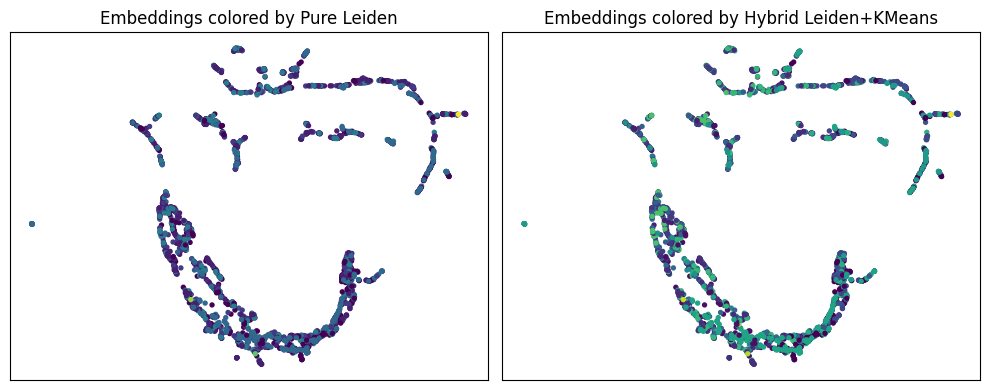
\includegraphics[width=\textwidth]{Fig 3-Pure Leiden Colors.png}%
    }{%
    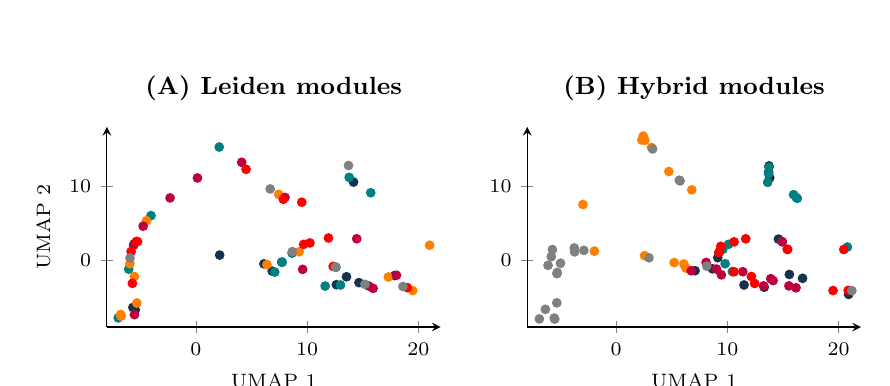
\begin{tikzpicture}
    \begin{groupplot}[
      group style={group size=2 by 1,horizontal sep=1.1cm},
      width=0.48\textwidth,height=0.34\textwidth,
      axis lines=left,tick label style={font=\scriptsize},
      label style={font=\scriptsize},title style={font=\small\bfseries},
      xlabel={UMAP 1},ylabel={UMAP 2},
      xmin=-8,xmax=22,ymin=-9,ymax=18,
      scatter/classes={a={navy},b={teal},c={orange},d={purple},e={red},o={gray}}
    ]
    \nextgroupplot[title={(A) Leiden modules}]
      \addplot[only marks,scatter,mark size=1.55pt,scatter src=explicit symbolic]
      coordinates {
      (-5.55,2.22)[a] (17.86,-2.05)[a] (7.72,-0.25)[a] (2.14,0.71)[a] (6.86,-1.46)[a] (14.17,10.56)[a] (13.54,-2.22)[a] (14.66,-3.01)[a] (-5.66,-6.36)[a] (6.12,-0.48)[a] (12.63,-3.29)[a] (-5.45,-6.69)[a]
      (-6.98,-7.77)[b] (-4.03,6.03)[b] (13.78,11.19)[b] (2.10,15.29)[b] (7.76,-0.25)[b] (7.09,-1.59)[b] (11.62,-3.47)[b] (12.59,-0.94)[b] (13.00,-3.33)[b] (-6.04,-1.19)[b] (8.65,0.97)[b] (15.72,9.12)[b]
      (-4.44,5.34)[c] (-6.74,-7.52)[c] (-5.53,-2.19)[c] (7.44,8.91)[c] (21.01,2.04)[c] (6.39,-0.57)[c] (9.28,1.15)[c] (17.30,-2.25)[c] (-6.76,-7.30)[c] (-5.93,-0.45)[c] (-5.31,-5.76)[c] (19.49,-4.08)[c]
      (15.93,-3.78)[d] (-5.60,2.03)[d] (4.12,13.23)[d] (15.52,-3.45)[d] (0.14,11.11)[d] (18.03,-2.02)[d] (-4.74,4.61)[d] (-2.32,8.42)[d] (8.01,8.48)[d] (9.60,-1.22)[d] (14.46,2.91)[d] (-5.52,-7.33)[d]
      (-5.82,1.19)[e] (7.86,8.24)[e] (19.00,-3.69)[e] (-5.24,2.52)[e] (12.34,-0.82)[e] (4.51,12.28)[e] (11.92,3.01)[e] (9.52,7.84)[e] (-5.35,2.54)[e] (9.69,2.15)[e] (10.25,2.35)[e] (-5.71,-3.11)[e]
      (18.61,-3.53)[o] (12.55,-0.89)[o] (8.67,1.17)[o] (13.72,12.79)[o] (15.20,-3.24)[o] (6.68,9.63)[o] (-5.92,0.32)[o]};
    \nextgroupplot[title={(B) Hybrid modules},ylabel={}]
      \addplot[only marks,scatter,mark size=1.55pt,scatter src=explicit symbolic]
      coordinates {
      (7.08,-1.40)[a] (15.56,-1.91)[a] (14.58,2.86)[a] (13.30,-3.63)[a] (13.73,12.74)[a] (9.13,0.35)[a] (13.70,11.92)[a] (13.80,11.13)[a] (16.75,-2.43)[a] (11.49,-3.33)[a] (8.65,-1.15)[a] (20.89,-4.60)[a]
      (13.61,10.52)[b] (10.10,2.16)[b] (20.78,1.79)[b] (13.73,12.56)[b] (16.27,8.36)[b] (10.44,-1.52)[b] (9.58,1.48)[b] (16.19,8.47)[b] (15.94,8.86)[b] (9.79,-0.46)[b] (13.69,11.69)[b] (14.91,2.52)[b]
      (4.73,11.98)[c] (2.30,16.24)[c] (5.21,-0.31)[c] (6.08,-0.50)[c] (2.43,16.77)[c] (2.54,0.63)[c] (6.79,9.51)[c] (3.17,15.22)[c] (-2.99,7.53)[c] (2.58,16.20)[c] (-1.96,1.24)[c] (6.27,-1.05)[c]
      (8.08,-0.29)[d] (11.38,-1.54)[d] (9.45,-1.96)[d] (15.41,1.47)[d] (15.52,-3.45)[d] (13.89,-2.48)[d] (13.25,-3.45)[d] (14.10,-2.73)[d] (16.16,-3.71)[d] (6.74,-1.41)[d] (14.93,2.50)[d] (9.01,-1.18)[d]
      (12.44,-3.12)[e] (11.64,2.90)[e] (10.59,-1.55)[e] (9.40,1.89)[e] (15.37,1.50)[e] (20.46,1.46)[e] (19.49,-4.08)[e] (20.85,-4.06)[e] (9.22,1.05)[e] (10.59,2.49)[e] (12.15,-2.19)[e] (9.28,1.15)[e]
      (5.67,10.81)[o] (-5.57,-7.80)[o] (-6.13,-0.68)[o] (-3.77,1.67)[o] (-5.53,-7.93)[o] (21.18,-4.09)[o] (3.27,15.03)[o] (-5.34,-5.74)[o] (-3.74,1.14)[o] (-5.30,-1.64)[o] (-5.84,0.49)[o] (-5.74,1.45)[o] (5.74,10.72)[o] (-2.91,1.34)[o] (-5.01,-0.40)[o] (2.94,0.34)[o] (-5.33,-1.80)[o] (8.14,-0.78)[o] (-6.91,-7.91)[o] (-6.37,-6.61)[o]};
    \end{groupplot}
    \end{tikzpicture}
    }
    \caption{Full UMAP projection of all 2,503 GAT feature embeddings, coloured by pure Leiden membership (left) and hybrid Leiden--K-means membership (right). Each point represents one RNA, DNA-methylation, or miRNA feature. The identical coordinates in both panels isolate the effect of relabelling; UMAP is descriptive, and all reported quality measures were computed in the original graph, embedding, or expression spaces.}
    \label{fig:umap}
\end{figure}

\subsection{Graph fidelity versus embedding compactness}

Table~\ref{tab:modulemetrics} and Figure~\ref{fig:metrics} quantify the central trade-off. Pure Leiden achieved weighted modularity 0.699. Hybrid refinement reduced it to 0.290, a 58.5\% decline, as expected because the second stage no longer optimizes the graph objective. The embedding silhouette improved from -0.085 to -0.061, but both values remained below zero and therefore indicate overlap or ambiguous assignment. The Davies--Bouldin index decreased from 35.19 to 25.94 (26.3\% lower), supporting improved embedding-space compactness under that measure.

The original expression space gave the opposite result. The silhouette coefficient changed from 0.025 for Leiden to -0.123 for the hybrid. Mean within-module correlation also decreased slightly, from 0.185 to 0.178, while mean between-module correlation increased from -0.013 to 0.018. Refinement therefore created smaller groups that were closer in the learned embedding but not more coherent in the untransformed molecular profiles.

\begin{table}[t]
\centering
\caption{Feature-module evaluation for the deterministic seed-42 run.}
\label{tab:modulemetrics}
\begin{tabular}{lrrl}
\toprule
Criterion & Leiden & Hybrid & Preferred direction \\
\midrule
Number of modules & 12 & 22 & task dependent \\
Largest module & 879 & 511 & task dependent \\
Weighted graph modularity & 0.699 & 0.290 & higher \\
Embedding silhouette & -0.085 & -0.061 & higher \\
Embedding Davies--Bouldin & 35.19 & 25.94 & lower \\
Expression silhouette & 0.025 & -0.123 & higher \\
Mean within-module correlation & 0.185 & 0.178 & higher \\
Mean between-module correlation & -0.013 & 0.018 & lower \\
\bottomrule
\end{tabular}
\end{table}

\begin{figure}[t]
    \centering
    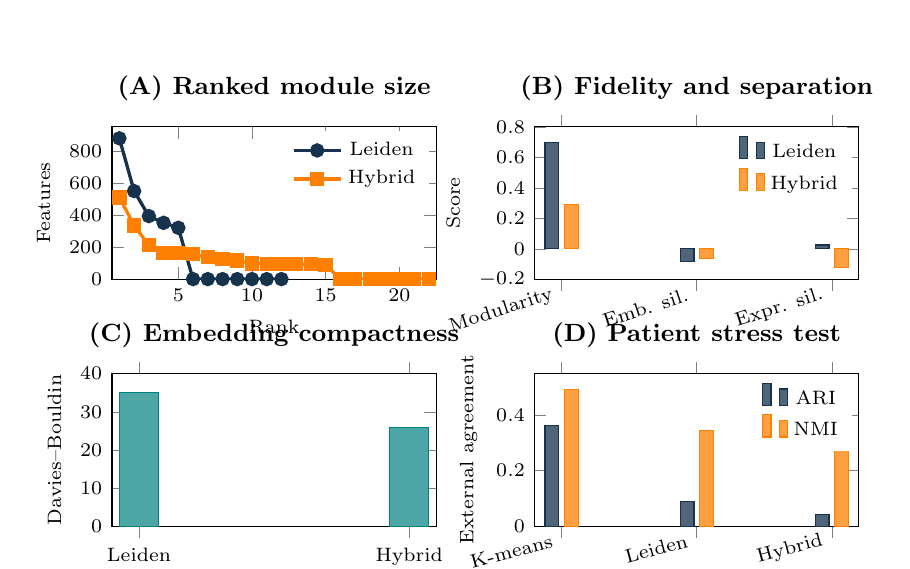
\begin{tikzpicture}
    \begin{groupplot}[
      group style={group size=2 by 2,horizontal sep=1.25cm,vertical sep=1.2cm},
      width=0.47\textwidth,height=0.29\textwidth,
      tick label style={font=\scriptsize},label style={font=\scriptsize},
      title style={font=\small\bfseries},legend style={font=\scriptsize,draw=none}
    ]
    \nextgroupplot[title={(A) Ranked module size},xlabel={Rank},ylabel={Features},ymin=0,ymax=950,xmin=0.5,xmax=22.5]
      \addplot[navy,very thick,mark=*] coordinates {(1,879)(2,550)(3,394)(4,352)(5,321)(6,1)(7,1)(8,1)(9,1)(10,1)(11,1)(12,1)};
      \addplot[orange,very thick,mark=square*] coordinates {(1,511)(2,336)(3,212)(4,165)(5,163)(6,156)(7,137)(8,127)(9,117)(10,99)(11,97)(12,97)(13,95)(14,94)(15,90)(16,1)(17,1)(18,1)(19,1)(20,1)(21,1)(22,1)};
      \legend{Leiden,Hybrid}
    \nextgroupplot[title={(B) Fidelity and separation},ybar,bar width=5pt,ymin=-0.2,ymax=0.8,
      symbolic x coords={Modularity,Emb. sil.,Expr. sil.},xtick=data,x tick label style={rotate=18,anchor=east},ylabel={Score}]
      \addplot[fill=navy!75,draw=navy] coordinates {(Modularity,0.699)(Emb. sil.,-0.085)(Expr. sil.,0.025)};
      \addplot[fill=orange!75,draw=orange] coordinates {(Modularity,0.290)(Emb. sil.,-0.061)(Expr. sil.,-0.123)};
      \legend{Leiden,Hybrid}
    \nextgroupplot[title={(C) Embedding compactness},ybar,bar width=14pt,ymin=0,ymax=40,
      symbolic x coords={Leiden,Hybrid},xtick=data,ylabel={Davies--Bouldin}]
      \addplot[fill=teal!70,draw=teal] coordinates {(Leiden,35.19)(Hybrid,25.94)};
    \nextgroupplot[title={(D) Patient stress test},ybar,bar width=5pt,ymin=0,ymax=0.55,
      symbolic x coords={K-means,Leiden,Hybrid},xtick=data,x tick label style={rotate=15,anchor=east},ylabel={External agreement}]
      \addplot[fill=navy!75,draw=navy] coordinates {(K-means,0.363)(Leiden,0.089)(Hybrid,0.043)};
      \addplot[fill=orange!75,draw=orange] coordinates {(K-means,0.492)(Leiden,0.344)(Hybrid,0.340)};
      \legend{ARI,NMI}
    \end{groupplot}
    \end{tikzpicture}
    \caption{Quantitative comparison. (A) Ranked module sizes. (B) Graph modularity and silhouette coefficients. (C) Embedding-space Davies--Bouldin index. (D) ARI and NMI for the secondary patient-clustering stress test.}
    \label{fig:metrics}
\end{figure}

\subsection{Phenotype-associated module signals}

All five non-singleton Leiden modules and all 15 non-singleton hybrid modules exhibited module-eigengene differences across PAM50 groups after Benjamini--Hochberg correction. The strongest Leiden association was module 3 ($n=352$, $F=1012.83$, $q=6.11\times10^{-303}$); the strongest hybrid association was module 9 ($n=97$, $F=982.48$, $q=3.14\times10^{-298}$). In the recorded exploratory annotation, hybrid modules separated established PAM50-associated features: one module contained \textit{ESR1}, \textit{PGR}, and \textit{FOXA1}; another contained basal/proliferation-associated features including \textit{KRT5}, \textit{KRT17}, \textit{EGFR}, \textit{BIRC5}, and \textit{MKI67}.

These small $q$-values should not be read as external biological validation. The GAT target was constructed from feature--PAM50 association, so testing its derived modules against PAM50 is partially circular. The result confirms that the implemented pipeline retains the phenotype signal used during training; it does not establish new independent pathways or clinical subtypes.

\subsection{Patient-clustering stress test}

The mutual patient graph was highly fragmented under resolution 1.0: Leiden produced 197 communities and the hybrid 207, far more than the five PAM50 reference classes. K-means on 16-dimensional patient principal components achieved ARI 0.363 and NMI 0.492. Leiden achieved 0.089 and 0.344, respectively; the hybrid achieved 0.043 and 0.340 (Table~\ref{tab:patient}). Refinement further reduced ARI because it subdivided already over-partitioned communities. The result demonstrates that the clustering class runs on patient graphs, but not that the selected graph and resolution are suitable for patient stratification.

\begin{table}[t]
\centering
\caption{Secondary patient-clustering stress test against PAM50.}
\label{tab:patient}
\begin{tabular}{lrrr}
\toprule
Method & Clusters & ARI & NMI \\
\midrule
K-means on 16 PCs & 5 & 0.363 & 0.492 \\
Weighted Leiden ($\gamma=1.0$) & 197 & 0.089 & 0.344 \\
Leiden + local K-means & 207 & 0.043 & 0.340 \\
\bottomrule
\end{tabular}
\end{table}

\section{Discussion}

\subsection{Principal contribution}

The primary contribution is a tested clustering extension for BioNeuralNet. The class handles weighted graph conversion, deterministic Leiden execution, node--embedding alignment, and optional bounded refinement using a compact interface. This fills a practical gap between topology-first community detection and embedding-first clustering. It also exposes, rather than hides, the disagreement between those objectives.

The experiment shows that local K-means behaves as intended computationally: it reduces the size of dominant communities and improves the Davies--Bouldin index. However, it does not improve every quality criterion. Graph modularity and raw-expression coherence deteriorate, and the embedding silhouette remains negative. A journal-standard interpretation is therefore conditional: use pure Leiden when the inferred feature network is the primary scientific object; consider refinement when smaller embedding-defined modules are required, but demand independent validation before interpreting them as biological units.

\subsection{Implications for multi-omics feature discovery}

Feature-module discovery and patient stratification are related but distinct tasks. In the primary graph, nodes are RNA, methylation, and miRNA features, so a community is a set of molecular measurements with similar cross-patient profiles and graph neighbourhoods. Such modules can support later enrichment, module scoring, or supervised prediction. They are not patient subtypes. The patient stress test makes this distinction concrete: transferring the same community settings to a sparse mutual patient graph produces nearly 200 communities and weak PAM50 agreement.

The result also illustrates why no single clustering score is sufficient. Modularity evaluates graph structure but is biased toward the graph used to construct the partition. Silhouette and Davies--Bouldin depend on a chosen metric space and may disagree. ARI and NMI require reference labels and can penalize legitimate finer structure. Module--phenotype association is valuable only when the phenotype was not already used to learn the representation. A reliable workflow should specify the scientific object and validation criterion before selecting resolution.

\subsection{Limitations}

Several limitations constrain the biological conclusions.
\begin{enumerate}
    \item The analysis uses one processed TCGA-BRCA cohort and one deterministic GAT run. It does not quantify stability across bootstraps, seeds, cohorts, or graph-construction choices.
    \item PAM50 is a categorical variable, but the current BioNeuralNet embedding target correlates features with an integer encoding. This imposes an artificial order. Categorical association measures or one-vs-rest targets would be more appropriate.
    \item The RNA, methylation, and miRNA tables were concatenated without modality-specific weighting or network fusion. Cosine similarities may therefore reflect platform-specific preprocessing as well as biology.
    \item The non-mutual adjacency is row-normalized before an upper-triangle conversion to an undirected graph. A future implementation should symmetrize weights explicitly, for example by the mean or maximum of $A_{ij}$ and $A_{ji}$.
    \item The graph and resolution setting were chosen from an exploratory sweep. No held-out criterion or consensus procedure was used, and the hybrid threshold of 30 nodes and cap of three subclusters are heuristics.
    \item ANOVA against PAM50 is not independent because PAM50 guided GAT training. UMAP is likewise descriptive and cannot establish cluster validity.
    \item No pathway enrichment, survival analysis, treatment-response analysis, or external-cohort replication was available in the executable record. Such results are therefore not claimed here.
\end{enumerate}

\subsection{Future work}

The next development step should replace ordinal correlation with a categorical phenotype objective and separate representation learning from validation labels. Repeated graph construction and clustering under patient and feature bootstrap resampling would allow consensus modules and stability intervals. Modality-specific similarity graphs could be fused or connected through a multiplex representation rather than concatenated without weights. For patient clustering, graph connectivity and Leiden resolution should be tuned jointly, with isolated components reported and the number of communities constrained only through predeclared criteria. Biological evaluation should then use held-out gene sets, pathway enrichment with an explicit background universe, independent BRCA cohorts, and clinical outcomes not used during training.

\section{Conclusion}

This study adds weighted Leiden community detection and optional embedding-level refinement to BioNeuralNet and evaluates the extension on a three-layer TCGA-BRCA feature network. Pure Leiden produced fewer, graph-coherent modules; local K-means produced finer modules with lower embedding-space Davies--Bouldin dispersion but substantially weaker modularity and expression coherence. A separate patient experiment showed that untuned Leiden settings over-partitioned the patient graph and did not outperform K-means. The defensible contribution is therefore not a universally superior clustering algorithm or a new clinical subtype system. It is a reproducible multi-resolution clustering component, an explicit account of its objective trade-offs, and a clear basis for future stability and external-validation studies.

\section*{Data Availability}

The TCGA-BRCA source data are available through the NCI Genomic Data Commons at \url{https://portal.gdc.cancer.gov/}. The aligned processed cohort used here is distributed in the BioNeuralNet source repository. No restricted clinical data were used.

\section*{Code Availability}

The evaluated extension is available on the public \texttt{Extended\_Clustering\_Component} branch at \url{https://github.com/UCD-BDLab/BioNeuralNet/tree/Extended_Clustering_Component}. The exact regeneration reference is commit \texttt{3c1915dc62851875672636e91f04f1eb9f1faf81}. At that revision, the executable notebook is \path{bioneuralnet/clustering/CSCI5250TermProjectExtendingClustringComponent.ipynb}; the current branch also exposes the curated notebook as \path{bioneuralnet/clustering/leiden_notebook.ipynb}. The implementation and interface tests are in \path{bioneuralnet/clustering/leiden.py} and \path{tests/test_leiden.py}, respectively.

\section*{Ethics Statement}

This secondary analysis used publicly available, de-identified TCGA data and involved no new participant recruitment or intervention. Ethical approval and informed consent for primary TCGA data collection were handled by the contributing institutions and TCGA program.

\section*{Author Contributions}

M.B.: Conceptualization, methodology, software, formal analysis, investigation, visualization, and writing---original draft. M.A.S.: Conceptualization, supervision, project administration, validation, and writing---review and editing. N.Q.: Methodological review, validation, supervision, and writing---review and editing. N.B.: Methodological review, validation, and writing---review and editing. T.U.J.: Biological interpretation, validation, and writing---review and editing. All authors reviewed and approved the final manuscript.

\section*{Funding}

This work received no specific external funding.

\section*{Conflict of Interest}

The authors declare no competing interests.

\section*{Consent for Publication}

Not applicable. The manuscript contains no identifiable individual-level information.

\section*{Acknowledgments}

The author thanks Vicente Ramos and Farnoush Banaei-Kashani for guidance on BioNeuralNet and graph-based multi-omics analysis, and acknowledges the TCGA Research Network for generating and sharing the BRCA data.

\appendix
\section{Reproducibility Parameters}

\begin{table}[H]
\centering
\caption{Parameters fixed for the regenerated analysis.}
\small
\begin{tabular}{p{0.25\textwidth}p{0.68\textwidth}}
\toprule
Stage & Setting \\
\midrule
Feature selection & top 1,000 RNA; top 1,000 methylation; all 503 miRNA \\
Feature graph & cosine; $k=25$; non-mutual; no self-loops; row normalized \\
GAT & 4 layers; hidden dimension 64; ReLU; dropout 0.5 \\
Training & Adam; learning rate $10^{-3}$; weight decay $10^{-4}$; 100 epochs \\
Leiden & weighted RB configuration partition; $\gamma=0.25$; seed 42 \\
Hybrid & refine if $n_c>30$; $k_c\leq3$; K-means \texttt{n\_init}=10 \\
UMAP & neighbours 15; minimum distance 0.1; seed 42 \\
Patient graph & cosine; $k=15$; mutual; Leiden $\gamma=1.0$ \\
Patient representation & PCA, 16 components; K-means $k=5$ \\
Core software & NumPy; pandas; SciPy; scikit-learn; NetworkX; PyTorch; PyTorch Geometric \\
Clustering/visualization & igraph; leidenalg; umap-learn; Matplotlib \\
Artifact reference & BioNeuralNet commit \texttt{3c1915dc62851875672636e91f04f1eb9f1faf81} \\
\bottomrule
\end{tabular}
\end{table}

\begin{thebibliography}{99}

\bibitem{parker2009}
Parker JS, Mullins M, Cheang MCU, et al. Supervised risk predictor of breast cancer based on intrinsic subtypes. \textit{J Clin Oncol}. 2009;27:1160--1167. doi:\href{https://doi.org/10.1200/JCO.2008.18.1370}{10.1200/JCO.2008.18.1370}.

\bibitem{tcga2012}
The Cancer Genome Atlas Network. Comprehensive molecular portraits of human breast tumours. \textit{Nature}. 2012;490:61--70. doi:\href{https://doi.org/10.1038/nature11412}{10.1038/nature11412}.

\bibitem{wang2014snf}
Wang B, Mezlini AM, Demir F, et al. Similarity network fusion for aggregating data types on a genomic scale. \textit{Nat Methods}. 2014;11:333--337. doi:\href{https://doi.org/10.1038/nmeth.2810}{10.1038/nmeth.2810}.

\bibitem{wang2021mogonet}
Wang T, Shao W, Huang Z, et al. MOGONET integrates multi-omics data using graph convolutional networks allowing patient classification and biomarker identification. \textit{Nat Commun}. 2021;12:3445. doi:\href{https://doi.org/10.1038/s41467-021-23774-w}{10.1038/s41467-021-23774-w}.

\bibitem{schultesasse2021}
Schulte-Sasse R, Budach S, Hnisz D, Marsico A. Integration of multiomics data with graph convolutional networks to identify new cancer genes and their associated molecular mechanisms. \textit{Nat Mach Intell}. 2021;3:513--526. doi:\href{https://doi.org/10.1038/s42256-021-00325-y}{10.1038/s42256-021-00325-y}.

\bibitem{ramos2026}
Ramos V, Hussein S, Abdel-Hafiz M, et al. BioNeuralNet: a graph neural network based Multi-Omics network data analysis tool. \textit{Bioinformatics}. 2026;42(6):btag365. doi:\href{https://doi.org/10.1093/bioinformatics/btag365}{10.1093/bioinformatics/btag365}.

\bibitem{traag2019}
Traag VA, Waltman L, van Eck NJ. From Louvain to Leiden: guaranteeing well-connected communities. \textit{Sci Rep}. 2019;9:5233. doi:\href{https://doi.org/10.1038/s41598-019-41695-z}{10.1038/s41598-019-41695-z}.

\bibitem{reichardt2006}
Reichardt J, Bornholdt S. Statistical mechanics of community detection. \textit{Phys Rev E}. 2006;74:016110. doi:\href{https://doi.org/10.1103/PhysRevE.74.016110}{10.1103/PhysRevE.74.016110}.

\bibitem{velickovic2018}
Veli\v{c}kovi\'c P, Cucurull G, Casanova A, Romero A, Li\`o P, Bengio Y. Graph attention networks. In: \textit{6th International Conference on Learning Representations}; 2018. \url{https://openreview.net/forum?id=rJXMpikCZ}.

\bibitem{rousseeuw1987}
Rousseeuw PJ. Silhouettes: a graphical aid to the interpretation and validation of cluster analysis. \textit{J Comput Appl Math}. 1987;20:53--65. doi:\href{https://doi.org/10.1016/0377-0427(87)90125-7}{10.1016/0377-0427(87)90125-7}.

\bibitem{davies1979}
Davies DL, Bouldin DW. A cluster separation measure. \textit{IEEE Trans Pattern Anal Mach Intell}. 1979;PAMI-1:224--227. doi:\href{https://doi.org/10.1109/TPAMI.1979.4766909}{10.1109/TPAMI.1979.4766909}.

\bibitem{benjamini1995}
Benjamini Y, Hochberg Y. Controlling the false discovery rate: a practical and powerful approach to multiple testing. \textit{J R Stat Soc Series B}. 1995;57:289--300. doi:\href{https://doi.org/10.1111/j.2517-6161.1995.tb02031.x}{10.1111/j.2517-6161.1995.tb02031.x}.

\bibitem{mcinnes2018}
McInnes L, Healy J, Saul N, Gro\ss berger L. UMAP: Uniform Manifold Approximation and Projection. \textit{J Open Source Softw}. 2018;3:861. doi:\href{https://doi.org/10.21105/joss.00861}{10.21105/joss.00861}.

\bibitem{hubert1985}
Hubert L, Arabie P. Comparing partitions. \textit{J Classif}. 1985;2:193--218. doi:\href{https://doi.org/10.1007/BF01908075}{10.1007/BF01908075}.

\bibitem{strehl2002}
Strehl A, Ghosh J. Cluster ensembles---a knowledge reuse framework for combining multiple partitions. \textit{J Mach Learn Res}. 2002;3:583--617.

\end{thebibliography}

\end{document}
